%%=============================================================================
%% Methodologie
%%=============================================================================

\chapter{Methodologie}
\label{ch:methodologie}

%% TODO: Hoe ben je te werk gegaan? Verdeel je onderzoek in grote fasen, en
%% licht in elke fase toe welke stappen je gevolgd hebt. Verantwoord waarom je
%% op deze manier te werk gegaan bent. Je moet kunnen aantonen dat je de best
%% mogelijke manier toegepast hebt om een antwoord te vinden op de
%% onderzoeksvraag.

In dit hoofdstuk zal er meer uitleg gegeven worden over het opstellen van de verschillende proof of concepts en waarom voor bepaalde implementaties gekozen zijn. Hierbij zal ook besproken worden hoe een basis Host-based Card Emulation applicatie opgebouwd wordt.

\section{Beveiligingsmethodes}

Voor dit onderzoek werd er gekozen voor drie verschillende beveiligingsmethodes uit \ref{sec:Beveiliging} die verder uitgewerkt zullen worden als proof of concept. De drie gekozen beveiligingsmethodes zijn biometric factors, encryption en tokenization. Door het kiezen voor deze drie beveiligingsmethodes kan er al een mooie vergelijking gemaakt worden tussen één beveiligingsmethode op hardware niveau namelijk biometric factors (in dit geval vingerscan) en twee beveiligingsmethodes op software niveau. Voor het testen van de verschillende gekozen beveiligingsmethodes is er natuurlijk een Android applicatie nodig waarbij het simuleren van een smartcard geïmplementeerd is aan de hand van Host-based Card Emulation. Google heeft een groot aanbod aan voorbeeld applicaties waarin verschillende technieken geïmplementeerd zijn via de best practices, waaronder ook een applicatie waarin HCE geïmplementeerd is die voor dit experiment gebruikt zal worden. In deze standaard applicatie zullen de drie beveiligingsmethodes geïmplementeerd en vergeleken worden. 


\section{Opbouw Host-based Card Emulation applicatie}
 
 Bij het ontwikkelen van een Host-based Card Emulation applicatie moeten er een paar dingen aangepast worden in de AndroidManifest en er moet een Apdu service klasse aangemaakt worden. Wanneer een standaard "one activity" applicatie gemaakt is moeten er twee permissies toegevoegd worden in de Android Manifest, <uses-feature android:name="android.hardware.nfc.hce" android:required="true" /> en <uses-permission android:name="android.permission.NFC" />, de eerste permissie laat de applicatie toe om hardware HCE technologie te gebruiken en de tweede permissie laat het toe om de NFC technologie van het apparaat te gebruiken. De Apdu service moet ook gedeclareerd worden in de AndroidManifest zie \ref{fig:Manifest}. Bij de declaratie van de service wordt er toestemming gegeven aan externe applicaties om verbinding te maken met de service aan de hand van android:exported="true", de permissie android.permission.BIND\_NFC\_SERVICE zorgt ervoor dat enkel externe applicatie met deze permissie verbinding kunnen maken met de service.
 
 \begin{figure}
 	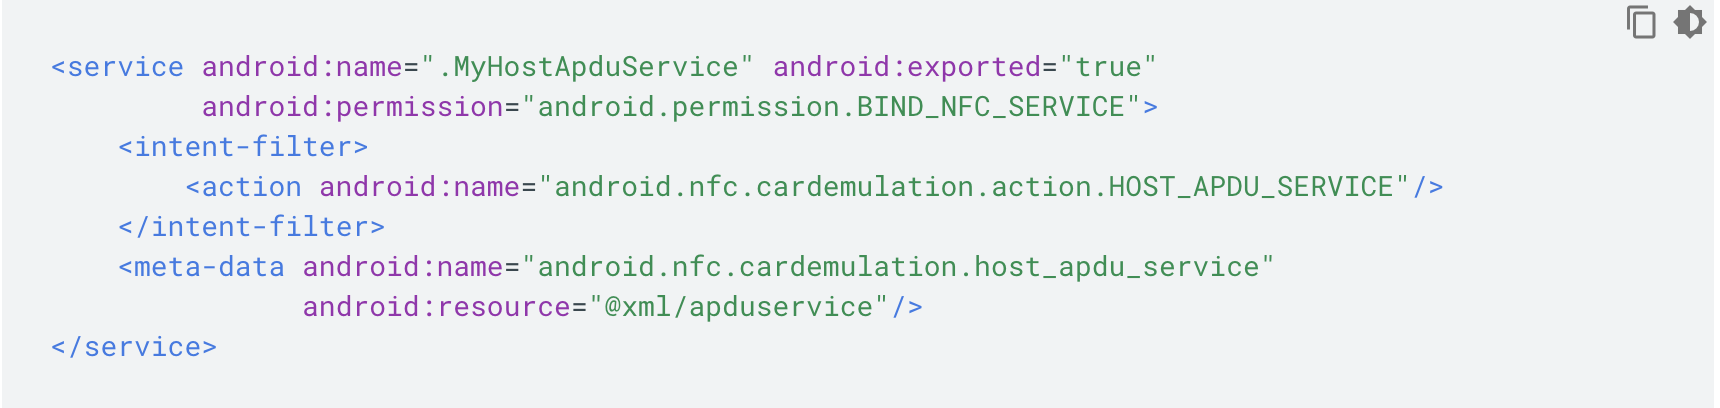
\includegraphics[width=\linewidth]
 	{img/ManifestService}
 	\caption{Service meta-data in AndroidManifest}
 	\label{fig:Manifest}
 \end{figure}

Bij het implementeren van de apdu service klasse wordt de klasse uitgebreid met de HostApduService klasse van android. De HostApduService klasse bevat twee abstracte methodes die overschreven worden in de eigen service klasse namelijk processCommandApdu en onDeactivated. De processCommandApdu methode wordt aangeroepen wanneer een NFC reader een APDU stuurt naar de apdu service en dan zal de service een APDU als antwoord terug sturen. Er moet wel rekening mee gehouden worden dat de processcommandApdu methode aangeroepen wordt op de main thread van de applicatie, wanneer het toestel dit niet aankan mag de main thread natuurlijk niet geblokkeerd worden. Wanneer de main thread het niet aankan moet de methode null teruggeven en een andere methode sendApduResponse die het antwoord op een andere thread terug zal sturen. De onDeactivated methode geeft terug of de apdu is teruggestuurd op de main thread of een andere thread wanneer de processCommandApdu wordt aangeroepen.